%\usepackage{subfig}

\chapter{Observations and Analysis}

In order to study this problem about the dynamics of Globular Clusters in our galaxy we need scientific data that allows us to build a model that fits our observations. Under supervision of proffesor Juan Carlos Mu\~noz Cuartas and with three other undergraduate students from the University of Antioquia a trip to the OPD (Pico dos Dias Observatory) was made to Brazil in May 2014, besides the observational experience of the students, the main purpose of the trip was to get important data for this project. We needed two sets of data corresponding to spectra and photometric images of the Globular Clusters

The spectroscopic data allows us to determine the velocity dispersion profile in the inner region of globular clusters while the photometric data allows us to study the surface brightness distribution for them. We can use all of this information to infer the properties of the globular clusters' mass distribution in order to build complete dynamical models and therefore infer the amount of dark matter present in the globular clusters (if there is any).

\section{Observational Procedures}

Our stay in OPD consisted of two days in the main dome for the spectroscopic data (using the Perkin-Elmer (P\&E) telescope with a 1.6m mirror and the Cassegrain Spectrograph) and four days in a smaller dome for the photometric data in the IAG telescope with a 0.6m mirror. In the following photograph, the domes of the observatory that we used for our observations:

\begin{figure}[h]
\centering
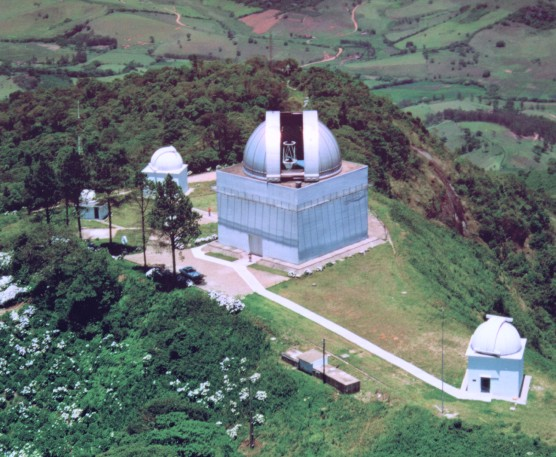
\includegraphics[width=10cm]{images/opd.jpg}
\caption{OPD observatory seen from the air, the big dome was used for the spectroscopic data and the small dome at the low right part of the photo for the photometric data.}
\end{figure}

\subsection{Spectroscopic Data}

The first two days (May 14th and 15th) we took the spectroscopic data in the telescope P\&E with a diameter of 1.6m. The main instrument was the Cassegrain spectrograph with a CCD Ikon-L camera and Filters BVR. The software we used was the recently installed software TCSPD which is built in a LabView environment for Windows (2010). Here's a photo of the telescope from inside the dome:

\begin{figure}[h]
\centering
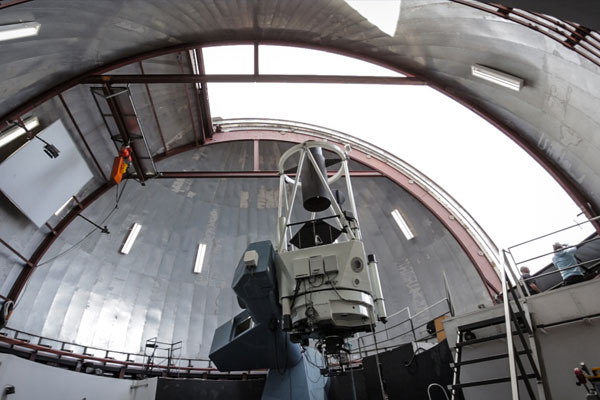
\includegraphics[width=10cm]{images/opd-spectrograph.jpg}
\caption{Perkin-Elmer telescope in the main dome in OPD used for the spectroscopic observations}
\end{figure}

We made the observations of dome flats, bias frames, comparison lamp frames, calibration stars and certain globular clusters of the milky Way organized by the best observation times using Simbad and Stellarium for the estimations of the coordinates and times respectively. We needed to keep an order of the observations to make the most of our observation time in OPD so we decided to organize our Globular Clusters in different groups or "chunks":

\begin{figure}[h]
\centering
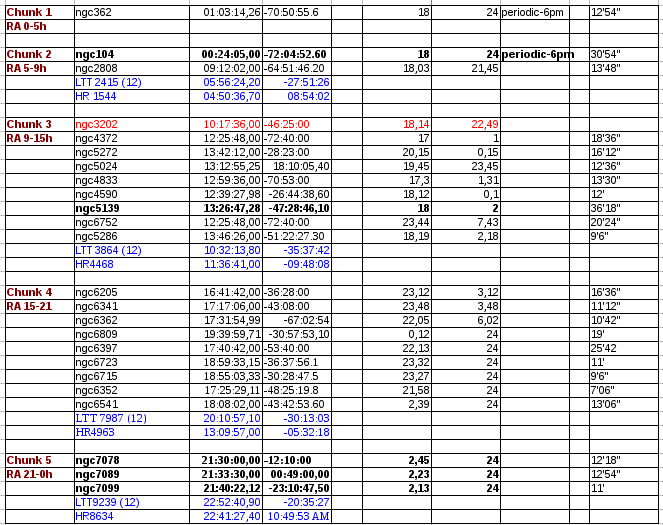
\includegraphics[width=10cm]{images/9.png}
\caption{Organized globular Clusters in groups for the proper times}
\end{figure}

Now, our set up configuration for the spectrograph was the following:

On May 14th, a diffraction grating of 900 lines per mm, a CCD IkonL and the central wavelength for the observations of 8500 Angstroms (with possibility of rotation of the slit 90°, +45° and -45°).we used the slit of 2.52" and obtained data for the globular clusters: NGC-5020, NGC-5272, NGC-4833, NGC-4590, NGC-5139, NGC-5286, NGC-6752, NGC-6397, NGC-6723, NGC-6715 and NGC-6541 using exposition times of 600 and 900 seconds. We also observed the calibration stars: HR-4963 and HR-4468 with 7 and 5 seconds. As it was the first day, we needed to be very careful in calibrating our instruments on order to have the objects in the right focus, we also made the rotation of the slit to use all the diffraction angles of the observations and our comparison lamps were of Ne-Ar.

On May 15th, we used the slit of 3.0", and used a central wavelength of 5500 Angstroms. This time we observed the following objects: NGC-2802, NGC-5024, NGC-4590, NGC-5139, NGC-5286, NGC-5272, NGC-6362, NGC-6397, NGC-6723, NGC-6502, NGC-6541, NGC-7078, NGC-7099, the stars HR-4468 and HR-7950 and we also observed Mars for pedagogical reasons. We used pretty much the same exposition times than the day before, this time though, our comparison lamps were or He-Ar. All the data we took was in FITS format (Flexible Image Transfer System).

\subsection{Photometric Data}

The photometric data were acquired in the next four days (from May 16th to May 19th) in the 0.6m IAG telescope in OPD. We used the Johnson system for the different filters which were easily shifted with the given software in the control computers. Here a picture of the telescope from inside the dome:

\begin{figure}[h]
\centering
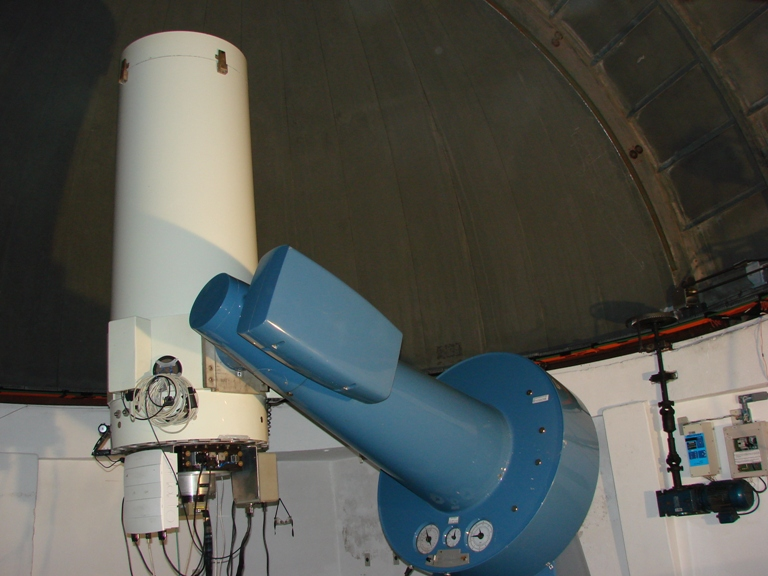
\includegraphics[width=8cm]{images/opd-photometry.jpg}
\caption{IAG telescope used for the photometric data}
\end{figure}

On May 16th, we took all the calibration images, consisting of 20 bias frames with an exposition time of 0,00001 seconds; also 22, 11, 11, 20 and 10 flat frames for the B,I,R,U,V filters respectively, their exposition times differed, for  U filter we took various frames of 60 and 30 seconds, for the B filter we took frames of 30 seconds each, 15s for I, 60s for R and 3s for V. We took our "focus" images to calibrate the instrument, and also various skyflats for all the filters. We targeted the following globular clusters and calibration stars in different filters: NGC5272, HR4961, NGC4590, NGC5139 AND NGC6397. The exposition time for the clusters was of 600 seconds and 2 and 4 seconds for the calibration star. 

May 17th was a terrible night for observations because the sky was too cloudy and the only useful data we could get were dome flats for the filters I,R and V that we could use instead of the bad dome flats of the first day. The reduction using the flats of another day are decent but this is not the ideal situation since mechanical movements of the instrument might slightly change its configuration and therefore it probably ends up with a reduction that is not the ideal one for science purposes.  

On May 18th we were more organized since we were getting familiar with the observations and therefore the data we got had little trouble in the upcoming analysis, even though the sky was clody at the end of the night. The science objects we observed were NGC5139, HR6308, NGC6723, NGC6541, NGC7078, HR7964 that were observed in the different filters. We got 20 bias frames, 14 dome flats in the vaious filters, but no skyflats. 

On May 19th we observed the Globular Clusters NGC5139, NGC4590, NGC6723, NGC6715, NGC6541, NGC6970, NGC5286, NGC639, NGC6541 and NGC6715, the calibration stars HR6386 and HR6386, 20 bias frames and flats for each filter.

\section{First step for Anaysis}

Our first goal in starting the analysis of all the relevant data was to organize all the images in order to reduce the time required to make the reductions. For every day the calibrations images, trash, calibration stars and objects were separated and they were given their correct names as they were in the headers and compared with the information sheets we filled at the time we were doing the observations. With the use of an account on the galaxy.udea.edu.co cluster, for proper and quicker analysis and safety of the data, all the files were correctly organized.

The next step was the reduction of all the images with the calibration files for each day, I started the photometric data to acquire certain skills in the use of IRAF because the reduction of the spectroscopic data was to be a little more complex and needed a deeper understanding of IRAF packages. 

I started with the cluster NGC-5139 ($ \Omega $ Centauri) because we got lots of data for that cluster in OPD and also because $ \Omega $ Centauri is a well known globular cluster since it is the largest in our galaxy and we can get a lot of information from the web. 

After the photometry of that cluster, the most relevant part of the reduction was to be made. The reduction and analysis of the spectroscopic data (May 14th and 15th), the methods for these reductions are quite special and are the most relevant part of the analysis because that is our most valuable information. The reduction was to be made very carefully because a good spectroscopic analysis depends upon a good reduction of the data. Just as with the photometric data, the first procedures were made for the Cluster NGC5139 to understand and master the techniques of the reduction and extractions.

\section{Photometry}

The photometry was made by the two traditional methods, PSF photometry and Aperture Photometry; even though the magnitudes calculated using both methods are quite different, the calibration constant between the two methods gave a good relation between them and made me trust the photometry results.

But first, the reduction of the data had to be done. The first step is to characterize the calibration images in order to see if there are any errors associated with the instrument or the way that the observations were made. By doing this we found that most of the flat-field images had brightness gradients in the corners and this was a problem we needed to correct because the increased value on the counts in these corners would affect the normalization of the super-flat that we would use to reduce the science data. Another systematic error that we found in all of our calibration and science frames was the presence of a strange water-looking figure at the top left corner of them, although it can be removed with the correct reduction, it obviously affected the CCD sensitivity by the time of the observations. Also, some filters showed a higher sensitivity to this systematic errors but at the end, the photometry could be made in the best data so that the dirty images don't affect our results.

In order to see how the data would be affected by the systematic errors we just mentioned, we produced a composite image using three images with the filters U,V and R and we did the same with the flats in those filters, the results are shown in the following figure:
  
\begin{figure}[h]
  \centering
  \begin{minipage}[b]{0.45\textwidth}
    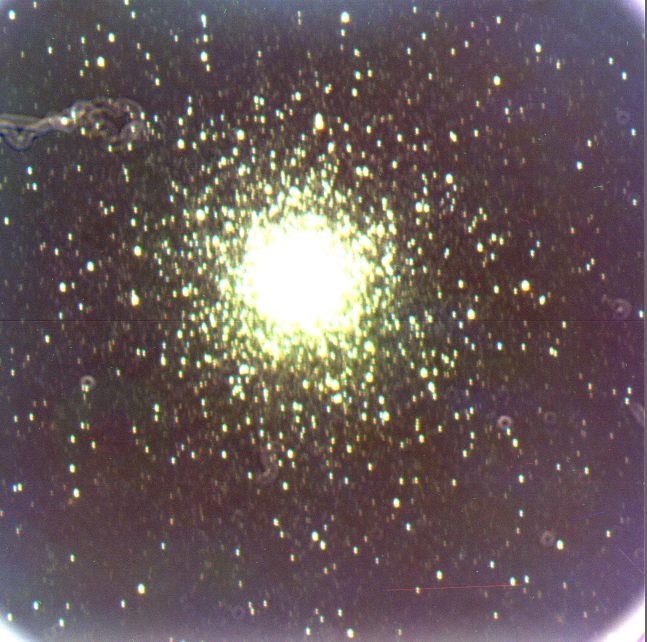
\includegraphics[width=\textwidth]{images/ngc_5139_dirty.png}
    \caption{Composite image of NGC5139 without being previously reduced}
  \end{minipage}
  \hfill
  \begin{minipage}[b]{0.45\textwidth}
    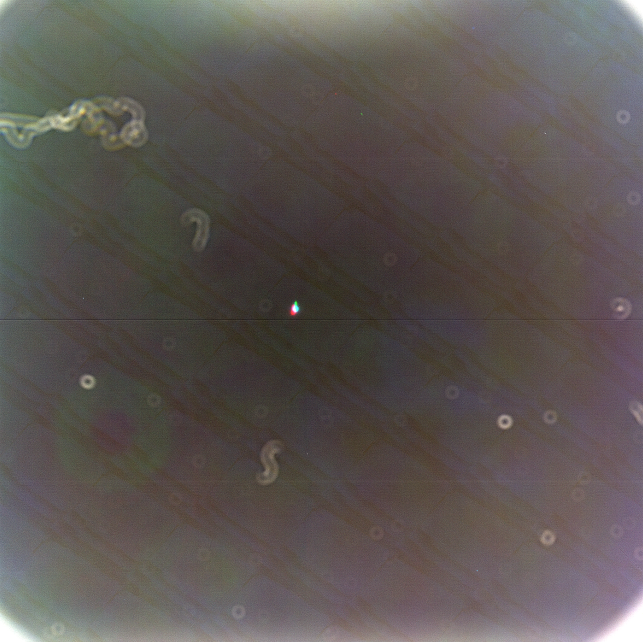
\includegraphics[width=\textwidth]{images/ruido.png}
    \caption{Composite image of the flats showing the noise that needs to be extracted}
  \end{minipage}
\end{figure}

What we can infer from these images is that the flat fields and the bias frames contain the same noise that the science data thus giving us a good result in the reduction.

Once all the characterization is made we can reduce our important data using IRAF following the conventional steps consisting of: 

- Building a Superbias: Zerocombine allows us to create the superbias using the median.

- Substracting the Superbias to every flat and science data: We substract the Superbias to every flat frame with no distiction on the filter, this is easily made using the task imarith, we also substract them from the original science images.

- Building Superflats: It is necessary to create a Superflat frame for each filter because the response of the CCD and will be different for different wavelengths, we use imcombine to do this and this time we use the mode for better results.   

- Divide the Superflats by the median: In order to normalize the flatfields we find the mode of each frame with imstatistics and then divide them by that value


\begin{figure}[h]
\centering
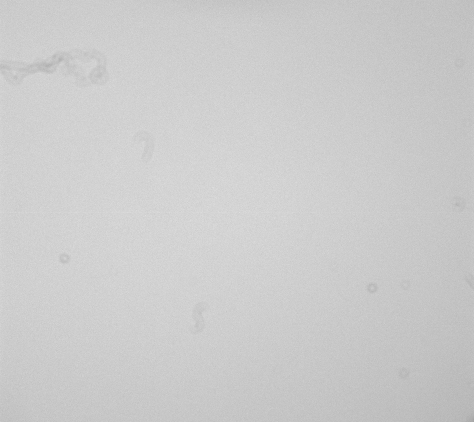
\includegraphics[width=8cm]{images/flat_I.png}
\caption{Example of one of the Normalized Superflats for the I filter}
\end{figure}

- Reduce the science data: Finally, we divide the original images of the clusters and stars (with the bias substractet) by the normalized Superflat to get the reduced images. This can easliy be made using the task imarith.

\subsection{Aperture Photometry}

Now that the reduction has been made and the corrections pixel by pixel have been applied, we can proceed to do the photometry using the simplest technique, known as Aperture Photometry which consists of adding up the pixel counts within a circle centered on each star of the cluster and subtracting the quotient of the per-pixel average value of nearby sky count divided by the number of pixels within the aperture. This will result in the raw flux value of the target object. This Aperture Photometry was done using the task Phot:

For stars in the NGC5139 cluster, one must choose a very small aperture of the sky because the surrounding stars contribute to the flux that needs to be extracted and they are very close to each other, as we can see in the following figure: 

\begin{figure}[h]
\centering
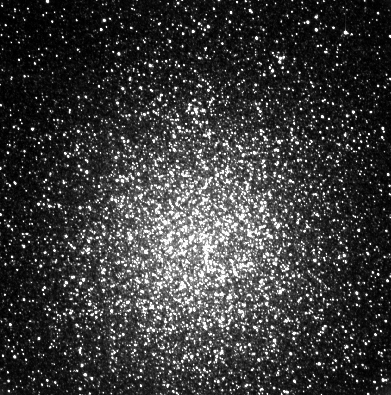
\includegraphics[width=8cm]{images/NGC5139_red.png}
\caption{One of our observations of NGC5139 in the V filter with an exposition time of 480 seconds}
\end{figure}

with the task imexamine I find a value for the FWHM of 6.4 which I will use to set the size of the apertures to do the photometry. For the size of the aperture containing each star I chose an aperture size of four times the FWHM of the point spread function associated to the stars because it is the one that best fits the photometry and minimizes the error (calculated for some stars pressing "a" with the imexamine task) and for the width of the aperture I chose I value of 2.5 times the FWHM.

Another important value to take into account before editing the parameters in phot is the medium value of the background on the sky, in the case of this cluster, I do an average on many different places in the background of the image and find a value of sigma for the image that is equal to 53.45.

Now the photometry is done by changing some of the parameters including the readnoise and the gain. In the fitskyparts task inside phot I set the inner radius called annulus to be 25.6 (4FWHM) and the intermediate width called dannulus of 16 (2.5FWHM). Finally, before running the task I make sure I do the photometry using various apertures because I want to see which one minimizes the errors. I set apertures to be 1FWHM, 1.5FWHM, 2FWHM, 2.5FWHM, 3FWHM, 3.5FWHM and finally run the task. The results of the magnitude found for one of the star as a funtion of the size of the aperture is displayed below:

\begin{figure}[h]
\centering
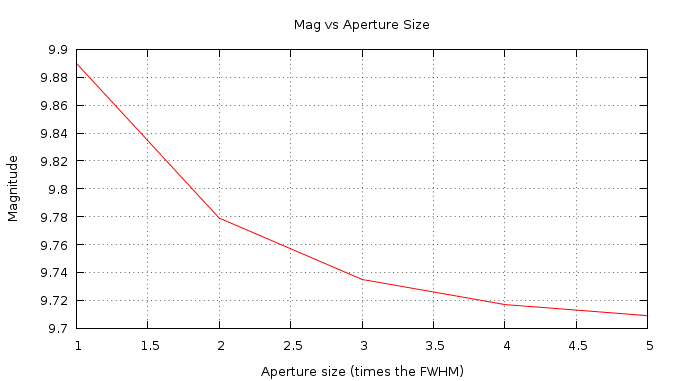
\includegraphics[width=12cm]{images/mag_vs_ap_size.png}
\caption{The magnitude decreases for bigger appertures}
\end{figure}

As we can see in the figure above, the magnitude of the chosen star in the cluster decreases for bigger appertures but so does the error because the space around the star is crowded of more stars and noice coming from the stars in the background so we infer that for crowded areas like this one the best choice is a small aperture. Although the results may not be as convincing, the use of another technique of photometry allows us to compare the results and see if the choice of a small aperture is a good way to fix or avoid the problem of the big noice of the background. For this purpose we use the technique of Point Spread Function (PSF) Photometry.

\subsection{PSF Photometry}

There exist many ways to count photons for an image taken with a CCD camera, but all of these ways obey the same principle of energy distribution in luminous objects. The point spread function for each of these objects is an assigned measure from the probabilistic distributions that approach quite well to the count of photons that one wants to do in the photometric analysis of astronomical images. The PSF photometry technique makes the most of the PSF of the obejtcs using certain packages and tasks in a slightly different way than aperture photometry.

When doing photometry in a very crowded field, such as a globular cluster (NGC5139 in this case), where the profiles of stars overlap significantly, one must use de-blending techniques, such as point spread function (PSF) fitting, to determine the individual flux values of the overlapping sources. 

This time, I made PSF photometry to some of the stars in the same cluster I started with (NGC5139), I chose bright ones that were relatively isolated to surrounding stars in order to make the estimations more accurate. First I use the same value of the PSF of some of those stars that I found doing the aperture photometry (6.4), this time the value of the sky is going to be higher because this value is going to determine the ammount of stars that the task daofind will select to do the photometry and I'm only interested in the brighter ones, a value of 2000 would filter out many of the fainter stars and the background. This values is using the standard deviation and making an average over many values found by the command "m" in the interactive mode of imexamine. 

After setting all the parameters of phot, daopars and findpars, I run daofind which will find the stars that match the criteria I mentioned above and will create a text file with the coordinates of those stars and will give to each star an ID.

The task \textit{tvmark} allows me to highlight the stars of the cluster in the display mode using the text file with the coordinates, and \textit{txdump} allows me to  put explicitly the coordinates of those stars in a text file that I use for the aperture photometry to make the first guess of the PSF of the stars.

The best way to correctly select the stars that will be used for the modelling of the PSF is by using the task pstselect that will select the stars that are well isolated using statistical techniques. 

Once the stars are selected, the next step is to use the task \textit{psf} which matches the point spread functions of the input images, by running this task, one can visualize how the PSF is modelled for each star and accept or decline the results to be stored, the interactive mode allows us to take the decision by analysing the modelling like the one we can see in the following image of the xterm:

\begin{figure}[h]
\centering
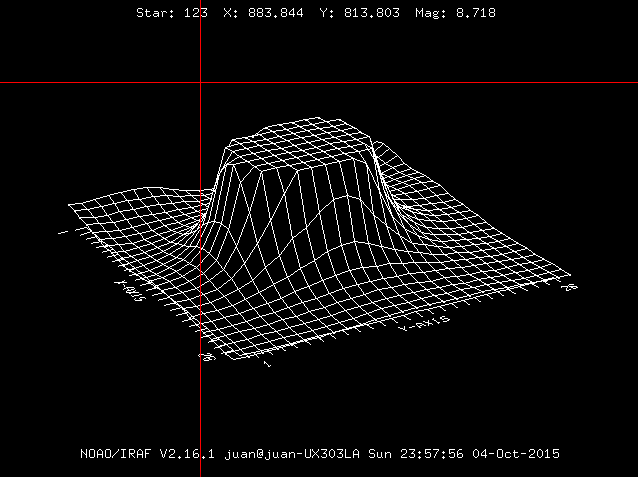
\includegraphics[width=10cm]{images/psf.png}
\caption{PSF modelling, the interactive mode allows us to accept of decline the result by pressing "a" or "d", in this case the PSF is not a soft curve with a gaussian behavior so it can probably be discarded}
\end{figure}

After running \textit{psf}, there will be created an image that contains the residuals of the psf modelling which can be seen like this:

\begin{figure}[h]
\centering
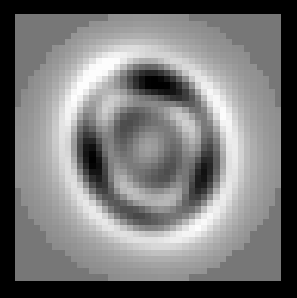
\includegraphics[width=5cm]{images/psf2.png}
\caption{T}
\end{figure}

With the task \textit{seepsf} another image will be created but this time it will actually look like a star:

\begin{figure}[h]
\centering
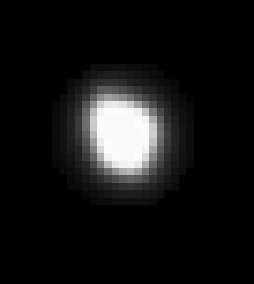
\includegraphics[width=5cm]{images/psf3.png}
\caption{T}
\end{figure}

Finally, after the modelling of the PSF was made, the task \textit{allsar} does the photometry of the cluster using the results we just stored in the current directory. The results of the PSF photometry gave us magnitudes smaller for those stars than the results given by the aperture photometry but there is a constant difference for all the stars which we can assume to be a calibration constant between the two methods. 

\section{Spectroscopy}

This is the most important part of the observational part of this project since the spectroscipc data has the most valuable information about the Globular Clusters and because our data were obtained in the largest and best telescope in OPD. Also, spectra of this kind is not easy to find in the scientific databases so we have important data to work with. The first spectroscopic procedures were also made for the $ \Omega $ Centauri cluster since we need to master the reduction and extraction techniques first in order to be able to start the scientific work about the mass modelling of the clusters.

\subsection{Spectroscopic Reduction}

The spectroscopic reduction is made by following some steps taking into account that we did not take any Skyflats so we need to create a response function using our dome flats. The steps are:

- First we make a Superbias combining all the bias frames and then we subtract it from all the lamp, targets and flat field frames.

- It was important to analize the flats to see which ones are saturated, we consider that values over 65,000 counts (using implot) show saturated data. The ones that we could trust for May 14th were ten images called flats\_0012 to flats\_0021.

- The pre-superflat is made using the median given the number of images.

- We need to make a trimming in all images because there are some regions in the images that show unexpected luminosity, this is probably due to border errors in the camera or the obturator time of relaxation. The zones we decided to cut were:

[0-100] and [575 to the end]

- A critical step is the creation of a response function, this is made by collapsing the pre-superflat to one column using \textit{blkavg}. The useful image for the creation of the Superflat is done by combining this column with \textit{blkrep}. This gives us an image that's uniformly distributed in the dispersion axis with the following IRAF commands.

blkavg MasterFlat.fits[1:475,*] AvgFlatCols 475 1

blkrep AvgFlatCols AvgFlatColsMaster 475 1

- The pre-superflat is now divided by the response function we created (AvgFlatColsMaster) and this gives us the Superflat that we will use to reduce our data.

- Finally, the task we use to remove the cosmic rays is \textit{lacos}, and it gives very accurate results, as it shows the "mask" image with the removed cosmic rays.

The vertical axis of the spectra is the dispersion axis and the horizontal axis is the spatial separation between stars. To visualize the reductions we have the following figures taken from the dirty and reduced NGC5139 spectrum (Day of observation May 14th):

\begin{figure}[h]
  \centering
  \begin{minipage}[b]{0.45\textwidth}
    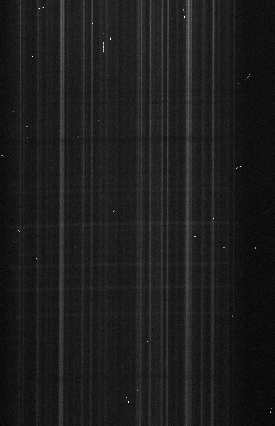
\includegraphics[width=\textwidth]{images/cluster_dirty.png}
    \caption{The dirty cluster spectrum has a small signal to noise ratio, besides border effects (such as a big gradient) that need to be trimmed and cosmic rays as we can see above}
  \end{minipage}
  \hfill
  \begin{minipage}[b]{0.45\textwidth}
    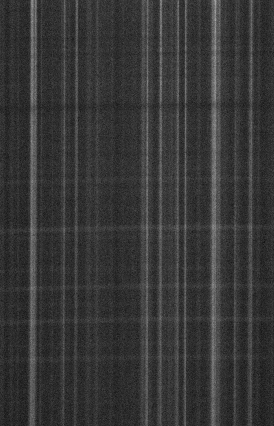
\includegraphics[width=\textwidth]{images/cluster_clean.png}
    \caption{The clean spectrum without the bad data at the borders that needed to be trimmed, with a higher signal to noise ratio and the cosmic rays removed, }
  \end{minipage}
\end{figure}

The images above are just a fraction of the whole image which is actually longer in the vertical direction, we chow only a fraction for visual purposes. As we did not take skyflats, some telluric lines are visible even in the reduced spectrum but this can be solved doing a correct calibration and carefully examining the extraction of the spectra of the stars.

\subsection{Extraction}

Once the reduction is ready, we can proceed with the extraction of the spectra of the calibration stars and also the spectra of the stars in the clusters, this procedure is made with the task apall.

Taking special care of correctly choosing the background, and with the following parameter configuration:

b\_number: 100

background: fit

weight: vairance

saturate: 65215

rdnoise: 6

gain: 1

Interactively, one must choose very precisely the background regions to extract the spectrum and do the fitting routines with different orders until the best results are reached.

The extraction of the spectrum for the calibration lamps is done with apsum, which is very similar to apall. For an individual star of the cluster, the extracted spectrum looks like this:

\begin{figure}[h]
\centering
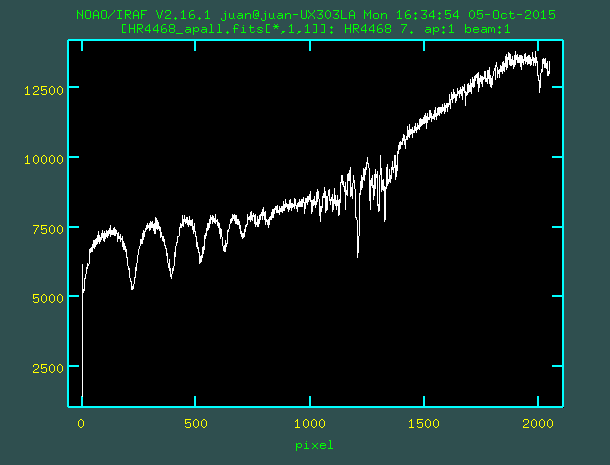
\includegraphics[width=8cm]{images/calib_star_apall.png}
\caption{T}
\end{figure}

\subsection{Wavelength Calibration}

The wavelength calibration is made many tasks of IRAF like Identify, Refspec and Dispcor. First, with identify I use the interactive window in IRAF to select some prominent lines in the spectrum and assign them their correct wavelength using the theoretic spectrum of the lamp. In this case our calibration lamps were Ne-Ar (for May 14th) and He-Ar (for May 15th)  and OPD observatory provided us the theoretic distribution of emission lines of them.

Using "m" to select the larger lines and typing the wavelength, the task creates a file stored in a new folder "database" with the pixels with their corresponding values in units of Angstroms. After that, the targets were to be calibrated with these files so it is necessary to edit their header to assign them the reference frames. It is enough to change the REFSPEC1 image header on each lamp file in order to do the wavelength calibration. 

The task that actually does the calibration on wavelength is dispcor, it is only necessary to run the task over all the targets with their own calibrated arc to get the calibrated spectrum which is the useful and important file to make the analysis of the width of the lines and their redshift.

\begin{figure}[h]
\centering
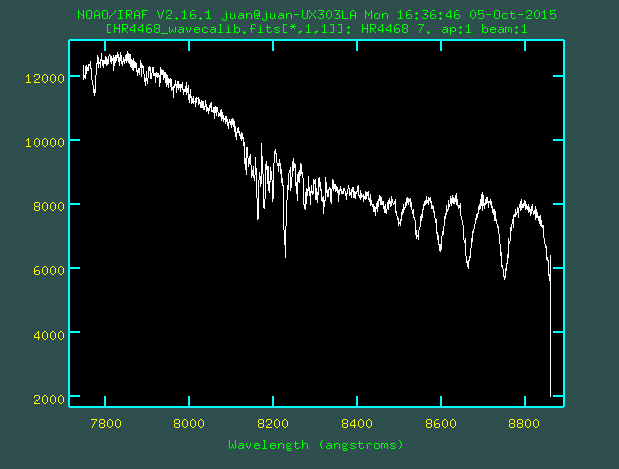
\includegraphics[width=8cm]{images/calib_star_wave.png}
\caption{T}
\end{figure}

\subsection{Flux Calibration}

The aim is to calibrate the CCD chip response, spectrograph+telescope throughput and allow for atmospheric extinction. The result is a spectrum as observed from outside the atmosphere with an ideal uniformly sensitive detector+telescope+spectrograph. Basically, what the flux calibration does is, it takes from a tabular compilation the energy distribution of the standard star, it corrects this energy distribution for wavelength-dependent atmospheric extinction, it compares it to the energy distribution of the observed spectrum and derives from such a comparison the function that gives the response of our system for every wavelength.

The flux calibration takes place in three parts: Calibrating from the standard star, calculating the sensitivity function of the instrument, and finally, applying the calibration to the spectra. We will use the task observatory to determine observatory parameters, standard to flux calibrate each standard star, and sensfunc to finally determine the wavelength response and the solution will be applied to the spectra by the task calibrate.

In the first part, the calibration is made with one of the stars that are already included in IRAF, there are many stars so there's quite a good amount of options to choose. So the first task is the task standard. The observatory parameter is specified as LNA which is in IRAF's database. 

\textbf{The task standard}

The task standard determines calibration pass-bands and writes them to a file called std. The thrick here is to specify the location of the the input extinction and flux calibration files. To do that, I edit the parameters of standard with the following routes:

Extinction file:                              onedstds\$/ctioextindt.dat

Directory containing calibration data:   onedstds\$ctionewcal/

Starname in calibration list:                l9239

Where I chose the Star l9239 because it has the spectral range that we use in our calibration Stars. And running the task interactively would be enough for this step.

\textbf{The task sensfunc}

Standard task just recorded response of each standard star so the next step is to put the results together and find a proper wavelength dependence of instrumental sensitivity and atmosphere transparency using the task sensfunc. It creates an image with a default name sens.0001. IRAF needs to have some general idea of atmospheric extinction before to start, so I set again extinct onedstds\$ /ctioextinct.dat.

Now, running the task interactively and taking into account that the function used to fit the instrumental response will be usually of very high order. A good idea is to use spline3 fitting (:function spline3) with some 20 pieces, i.e. (:order 20).
Finally q exists the sensfunc task and writes the sens.0001 image.

\textbf{The task calibrate}

The solution to each star to be calibrated is done with the task calibrate. Editting the parameters of calibrate to set the appropriate extinction table: extinct onedstds\$ /ctioextinct.dat would be enough for this purpose. The task is run over all the wavelength calibrated spectra which had their airmass and other parameters appropriately set by the eso.set procedure. And finally it gives the flux-calibrated spectra ready for the relevant analysis concerning radial velocities.

After the flux calibration, I notice that the extremes of the spectra have irregularities but that can be cut because they don't have any relevant information.

For the star calibration I cut from 0 to 45 and from 1860 to the end, using imcopy:

\begin{center}
imcopy flux\_calib\_star\_fits[45:1860,*] cut\_flux\_calib\_star.fits
\end{center}

\begin{figure}[h]
\centering
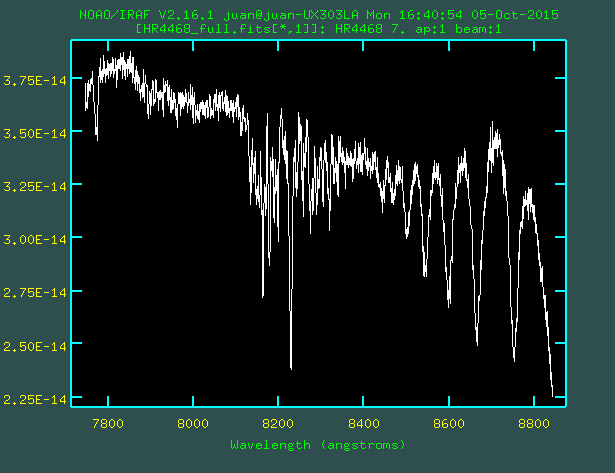
\includegraphics[width=8cm]{images/calib_star_flux.png}
\caption{T}
\end{figure}

In order to normalize the spectrum, first I find the maximum value in the spectrum using minmax and then I divide the whole image by this value.

Now, to create the Ascii table from the spectrum I need to first convert my image to a 1D image using the task scopy and setting format=onedspec

Now, with the image ready in 1D, I use the task wspectext to create the Ascii table like this:

\begin{center}
wspectext ready\_flux\_star.0001.fits normal\_cut\_flux\_star\_calib.txt
\end{center}

\section{RVSAO and radial velocity determination}